% ファイル名は「番号_タイトル.tex」
% 番号はNotionを参考
\section{受付}  % 割り振りの名前を記入

\subsection{場所・人員配置}
\begin{table}[h]
  \centering
  \begin{minipage}[t]{0.48\columnwidth}
    \centering
    \caption{場所・該当グループ}
    \begin{tabular}{cl}
      \hline
      場所 & K101 \\
      \hline
      グループ & 全員 \\
      \hline
    \end{tabular}
  \end{minipage}
  \begin{minipage}[t]{0.48\columnwidth}
    \centering
    \caption{役割分担}
    \begin{tabular}{ll}
      \hline
      \multicolumn{1}{c}{役割} & \multicolumn{1}{c}{担当者} \\
      \hline
      受付1 & 田中 \\
      受付2 & 丸山 \\
      受付3 & 岩村 \\
      受付4 & 納富 \\
      \hline
    \end{tabular}
  \end{minipage}
\end{table}

\subsection{詳細タイムスケジュール}
\vspace{0.5em}
\fontsize{8pt}{12pt}\selectfont

\begin{longtable}[c]{|p{.04\textwidth}|p{.2\textwidth}|p{.25\textwidth}|p{.45\textwidth}|}
  \caption{スケジュール} \\
  \hline
  \multicolumn{1}{|c|}{時間} & \multicolumn{1}{c|}{担当} & \multicolumn{1}{c|}{内容} & \multicolumn{1}{c|}{備考} \\
  \hline
  \endfirsthead

  \hline
  \multicolumn{1}{|c|}{時間} & \multicolumn{1}{c|}{担当} & \multicolumn{1}{c|}{内容} & \multicolumn{1}{c|}{備考} \\
  \hline
  \endhead

  \hline
  \endfoot

  \hline
  \endlastfoot

  \begin{tpacol}
    13:00
  \end{tpacol}&
  \begin{tpbcol}
    受付担当全員
  \end{tpbcol}&
  \begin{tpccol}
    受付開始
  \end{tpccol}&
  \begin{tpdcol}
    新入生が来たら名簿に印をつける
  \end{tpdcol}\\

  \begin{tpacol}

  \end{tpacol}&
  \begin{tpbcol}
    受付担当
  \end{tpbcol}&
  \begin{tpccol}
    班案内
  \end{tpccol}&
  \begin{tpdcol}
    新入生に所属班を伝え，スクリーンを参考に着席案内
  \end{tpdcol}\\

  \begin{tpacol}

  \end{tpacol}&
  \begin{tpbcol}
    受付担当
  \end{tpbcol}&
  \begin{tpccol}
    人数集計
  \end{tpccol}&
  \begin{tpdcol}
    各班の人数をカウント
  \end{tpdcol}\\

  \begin{tpacol}
    13:30
  \end{tpacol}&
  \begin{tpbcol}
    受付担当
  \end{tpbcol}&
  \begin{tpccol}
    受付終了・報告
  \end{tpccol}&
  \begin{tpdcol}
    イベント班へ参加人数と各班人数を報告後，待機
  \end{tpdcol}\\

\end{longtable}
\normalsize

\subsection{準備物品}
\begin{table}[h]
  \centering
  \caption{物品}
  \begin{tabular}{lrl}
    \hline
    \multicolumn{1}{c}{物品} & \multicolumn{1}{c}{数量} & \multicolumn{1}{c}{使用用途・備考} \\
    \hline
    机 & 4 & 教卓側出入り口付近に設置 \\
    名札 & 新入生人数分 & 受付時に配布・確認 \\
    名簿 & 1 & 出欠確認用 \\
    \hline
  \end{tabular}
\end{table}

\subsection{備考}
\begin{figure}[H]
  \centering
  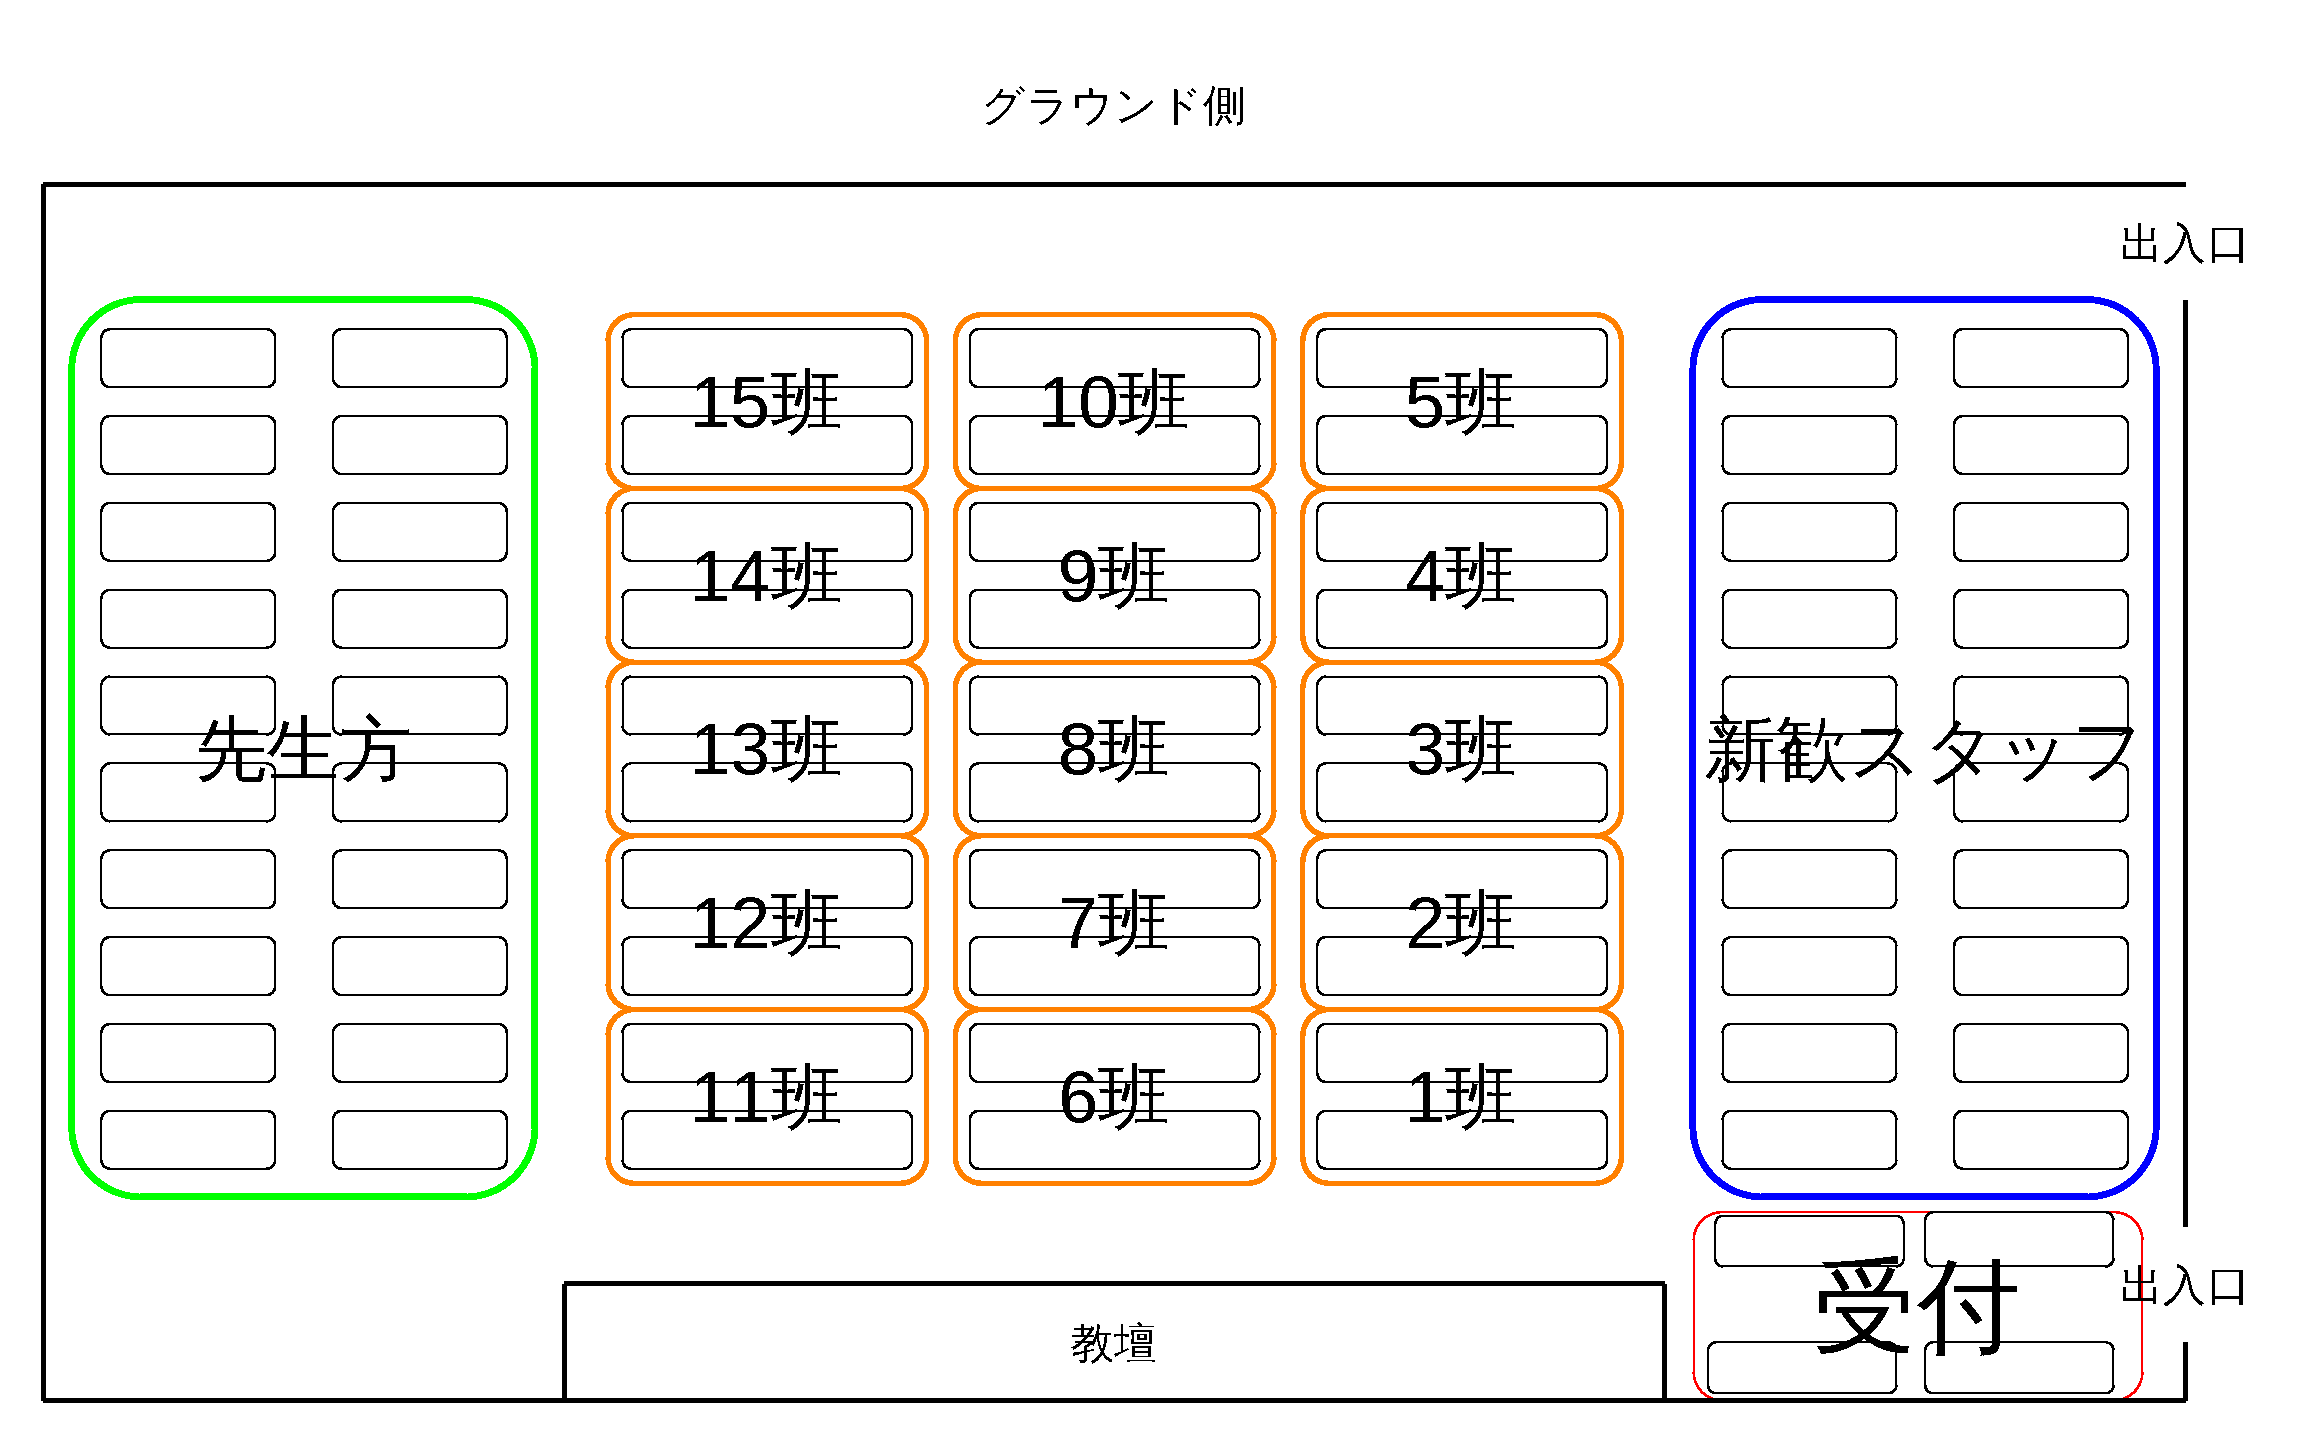
\includegraphics[width=1\linewidth]{document/3_Deta/配置.pdf}
  \caption{教室の様子}
\end{figure}
